\chapter*{Introduction}

\begin{figure}[h]
    \captionsetup{labelformat=empty}
    \hspace{\stretch{1}} 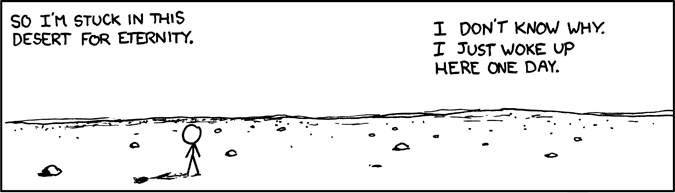
\includegraphics[width=0.75\textwidth]{xkcd/xkcd1.png}
    \caption*{\hspace{\stretch{1}}  Randall Munroe, \emph{A Bunch of Rocks} (part 1 of 9), \texttt{xkcd.com/505/} }
\end{figure}




%In the beginning there was a plan. A vague plan, a few open ideas on what my thesis should cover and what topics I was about to dedicate the next few years of my life to. There would be quanta involved, of that I was sure. There would be entanglement issues, towards which my undergraduate thesis led me. There would also be travels, substantial time spent on another continent, which I welcomed. Apart from that, no particular goal, no traced out road to follow, no limits to what I could achieve. Well, in theory anyway.

%Let's face it, there was no plan. I was free to choose a face and a body for my thesis. That freedom allowed me to hop from problem to problem, to expand my knowledge into several fields of the quantum theory, led by the random or not so random ideas that were flourishing around me. A lector will not find in this work six chapters walking together hand in hand towards a grand conclusion, but rather a set of several subsystems which are definitely interacting with their first neighbors, but with not much further. Nonetheless, those chapters form a strange molecule that I am happy to to call my thesis.

Quantum entanglement is by far the most intriguing feature of quantum mechanics compared to any other classical theory. It plays a fundamental role in every apparent paradox or counter-intuitive consequence of quantum theory. Its mind-blowing properties have many, many application in a very large range of fields. In spite of this incredible success, characterization and classification of entanglement in a general state is still an open question of the quantum theory. That is the very issue that motivated this work. The first two chapters of this thesis introduce entanglement criteria of various domains of application that contribute to this search of entanglement characterization. For the rest of the thesis, we set aside the mathematical considerations and consider the fascinating problem of experimentally producing entanglement in physical systems and more particularly in systems of cold atoms.  This entanglement production must come from ingredients  available in the laboratories today: lasers, cavities, cold atoms in gazes or isolated and, most importantly, interatomic interactions. In chapters~\ref{ch-3} to~\ref{ch-5}, we consider dipole interactions between atoms and the phenomenon of dipole blockade as a mean to produce entanglement in systems of two or more atoms. In chapter~\ref{ch-6}, we explore the many possibilities of cavity quantum electrodynamics.  Every chapter just about stands on its own and will be duly self-introduced and placed into its context in the literature, but we present them briefly here.

Chapter~\ref{ch-1} is devoted to \textit{Multipartite Entanglement Criterion from Uncertainty Relations}. In this chapter, we describe a criterion which can experimentally detect the presence of entanglement in a wide variety of quantum states. That criterion is the love child of two great concepts in quantum mechanics, the Schr\"odinger-Robertson inequality (SRI) and the positive partial transpose (PPT) criterion. The SRI is a generalization of the even more famous Heisenberg inequality and describes how the product of the variances of two non-commuting operators can never be smaller than some particular minimal value. The PPT criterion shows that under the action of a particular mathematical operation, the partial transpose, the density matrix of a separable state must remain a physical quantity, whereas the density of an entangled state might very well not do so. By bringing those two concepts together, we were able to define the Schr\"odinger-Robertson partial transpose criterion. This criterion dictates that the product of the variances of two observables modified by the partial transpose operation will always be bounded by a minimal value when acting on a separable state. An entangled state, however, might violate the inequality, a certain sign of its entanglement. We show that in order to satisfy some constraints due to the SRI and the PPT criterion, the observables must obey some specific conditions and we show their general form for bipartite systems. We go on proving that our entanglement criterion is necessary and sufficient for any pure bipartite state or even any pure three-qubit state. We test its performances on a large variety of systems, harmonic oscillators, multi-photon polarization states, Schr\"odinger cat states and multipartite mixed states.

Chapter~\ref{chap-conc} is devoted to \textit{Concurrences for $N$-qubit Systems}. In that chapter, we present another entanglement criterion inspired from the criterion of the concurrence. The concurrence is a mathematical criterion that not only detects entanglement in two-qubit states, but also quantifies the amount of entanglement for pure states or mixed states. We start the chapter by introducing the concurrence. Next, we give a series of nine conditions that a pure three-qubit state must obey to be separable. We prove that those conditions are necessary and sufficient conditions to entanglement with a formalism that can easily be generalized to systems of more qubits. We then take advantage of those conditions to define concurrences for tripartite pure states. We show that those quantities are linked to other values used to evaluate tripartite entanglement. Using the formalism of the original concurrence, we prove that our concurrences can also be evaluated easily on mixed states. Any non-zero concurrence is a sure sign of entanglement. We finally test our criterion on different mixed states and find encouraging results. In the second part of the chapter we generalize the whole process to systems of $N$-qubits. We show that the number of conditions to separability grows very much with the number of qubits, but we can still compute them and we define generalized concurrences, which are necessary and sufficient conditions for entanglement in pure states. We finally prove that they may also be applied on mixed states.

Chapter~\ref{ch-3} is devoted to \textit{Entanglement, Antibunching, and Saturation Effects in Dipole Blockade} and leads the path of quantum information theory into the domain of quantum optics. In this chapter, we study the interaction of two identical two-level atoms immersed in a resonant laser field. The Hamiltonian model for the interaction is specifically chosen to describe the dipole blockade effect. In a blockaded system, one atom in its excited states prevents, with some degree, the other atom to get excited. The interest of such an interaction is the production of entanglement. Indeed, a system of two independent atoms can never be entangled by a laser, however a blockaded system is constrained to deal only with the ground state and a coherent superposition of ``first atom excited, second not excited'' and of the opposite situation and such a superposition is shown to carry maximal entanglement. After introducing our Hamiltonian, we introduce the master equation which modelizes dissipation effects in the system, allowing us, after a few considerations about the non-interactive case, to compute the time evolution of the system. We measure the concurrence as well as a quantity able to estimate the blockade on time-evolving states. We show that our model describes the dipole blockade well and also that the strengthening of the laser power has the effect of lifting said blockade. Then, we study the equilibrium case, the steady state of the system and we give its analytical description as well as an analytical expression of its concurrence. That expression allows us to tune the laser power in order to maximize the amount of entanglement for a given interaction strength. Finally, we study another way to experimentally show the blockade effect, the photon-photon correlation.

Chapter~\ref{ch-4} is devoted to \textit{Dipole Blockade and Entanglement in Three-Atom Systems} and generalizes the Hamiltonian model for the dipole blockade effect on systems of three two-level atoms. We start by introducing the model, along with a particular basis which takes advantage of the possible symmetries of the system. We also define quantities which measure the blockade effect, which can now be considered for a particular pair of atoms or for the three of them altogether. We then consider several different cases of interaction:  no interaction between the atoms, interaction between only two, same interaction between all atoms and aligned atoms with interaction between first neighbors only. For each case, we give an analytical value of the steady state and study their blockades. We observe blockades in the different cases with varying amplitudes except for one particular case where antiblockade is observed. After that, we study the two-atom concurrences by tracing out one atom and find that bipartite entanglement is weakened by the presence of a third interacting atom. Finally, we study tripartite entanglement using the three-qubit concurrences defined in chapter~\ref{ch-3} and find indications of bipartite entanglement in the system as well as genuine tripartite entanglement.

Chapter~\ref{ch-5} is devoted to \textit{EIT, Dipole Blockade and Dipole-Dipole Interaction}. In this chapter, we introduce the electromagnetically induced transparency (EIT). The EIT is a phenomenon taking place in multi-level systems excited by two non-resonant lasers, the pump and the probe, where under some conditions the absorption of the probe laser is cancelled for a specific window of frequency. We start by quantifying this effect with the steady state of a single three-level atom and check established results. Then we investigated what would happen to the EIT if two atoms were to experience dipole blockade. We introduce our model Hamiltonian and master equation, check the eigenstates of the system with the probe laser turned off. Armed with those weapons, we measure the dipole blockade in the system as well as the effect on EIT. In the second part of the chapter we test the effects of another type of interaction, the dipole-dipole interaction. We introduce our model, Hamiltonian and master equation, find the eigenstates of the unperturbed system and compute the values of the dipole blockade and the effect on EIT in the steady state. We find a strong modification in the behavior of the EIT.

Chapter~\ref{ch-6} is the last chapter and is devoted to \textit{Cavity Mediated Two-Photon Processes in Two-Qubit Circuit QED}. In free space, two non-identical two-level atoms may not be simultaneously excited by a laser through a two-photon process. We explore the possibility that this inhibition, due to interference effects, can be beaten by placing the atoms in a single mode cavity. After briefly checking what happens in free space, we give our model Hamiltonian an master equation which modelize the different atomic frequencies, the cavity mode, the interaction between them, the laser field exciting the cavity modes and the dissipation effects such as the atomic spontaneous emission and the cavity losses. We first make an assumption on the atomic frequencies which allows us to diagonalize the unperturbed Hamiltonian and find the eigenvalues and eigenstates of the bare system. Then, using a perturbative approach, we find that  two-photon processes are indeed possible in such a system at some particular frequencies and we calculate the transition rates. We confirm our calculations by producing different atomic and photonic spectra in the steady state of the system. We find that the quality of the cavity has a strong effect on the structure of the spectra and induces behaviors not predicted by perturbation theory. In the last part of the chapter, we lift the constraint of the atomic frequency and confirm our results by numerically checking the same spectra for a most general configuration of the system. We also find a new feature of the system, the cavity induced transparency.

In the conclusion, we summarize all the results we were able to get and finally we give the appendices, which contain calculations not essential to the text as well as steady state results too imposing to fit in the chapters.
